\documentclass{assignmeownt}
\usepackage{listings}
\usepackage{amsmath}

% Set section counter and format
\setcounter{section}{2} % Start the section numbering from 2 so the next section will be 3


\coursenumber{05124265}
\coursetitle{Reinforcement Learning}
\title{Exercise 1}
\author{Tal Grossman, 201512282 , Inbal Cohen 211388491}
\date{28/05/2024}


\begin{document}
\maketitle
\thispagestyle{firststyle}
\section{Theory}
\subsection{Longest increasing subsequence}
We will use dynamic programming to find the length and elements of the longest increasing subsequence in a given list. The Python code is provided below (also attached as \textbf{3.1\_lis.py} in the Python files):

\begin{lstlisting}[language=Python, basicstyle=\tiny, caption={Python code for finding the longest increasing subsequence}]
def longest_increasing_subsequence(arr: List[int]) -> Tuple[int, List[int]]:
    Finds the length and elements of the longest increasing subsequence in a given list.
    It uses dynamic programming to solve the problem in O(n^2) time complexity.
    Args:
        arr (List[int]): The input list of integers.
    Returns:
        Tuple[int, List[int]]: A tuple containing the length of the longest increasing subsequence
        and the elements of the subsequence in the order they appear in the original list.
    n = len(arr)
    # dp[i] stores the length of the longest increasing subsequence ending at index i
    dp = [1] * n
    # prev[i] stores the index of the element before arr[i] in the longest increasing subsequence
    prev = [-1] * n  # init to -1 to indicate the start of the subsequence

    # iterate over the list to find the longest increasing subsequence by
    for i in range(1, n):
        for j in range(i):
            if arr[j] < arr[i]:
                if dp[j] + 1 > dp[i]:
                    dp[i] = dp[j] + 1
                    prev[i] = j

    max_len = max(dp)
    max_idx = dp.index(max_len)

    lis = []
    while max_idx != -1:
        # insert at the beginning of the list to maintain the order
        lis.insert(0, arr[max_idx])
        # move to the previous element in the subsequence
        max_idx = prev[max_idx]

    return max_len, lis
\end{lstlisting}

\subsection{Moses The Mouse}
\begin{enumerate}
  \item Moses goal is to find a policy that maximizes the total reward (cheese) collected from start position $(1,1)$ to $(M,N)$. 
  \newline
  To formulate the problem as a finite horizon decision problem we define the following:
    \begin{itemize} % spaces
    \item \textbf{\underline{state space:}}
    
    the state space represents all positions and configurations of Moses in the apt, i.e. the idx of the room.
    state is defined by $s = (i,j)$ where $i<=M$ is row idx and $j<=N$ is the column idx. so:
    \newline
    \begin{math}
        S=\{(i,j) \mid 1\leq i\leq M, 1\leq j\leq N\}
    \end{math}
    \item \textbf{\underline{action space:}}
    
    
    the action space $A$  which is actually it possible movements Moses can perform can be represented as 
    \begin{itemize} 
        \item \textbf{north} = from $(i,j)$ to $(i-1, j)$ if $i>1$  
        \item \textbf{east} = from $(i,j)$ to $(i, j+1)$ if $j<N$  
    \end{itemize}    
    so, $A = \{north, east\}$

    \item \textbf{\underline{cumulative cost function:}}
    \newline
    in our case, the cost function is actually a reward function where a room $(i, j)$ contains cheese. let $C$ be the set of states (rooms) with cheese, so:
    \newline
    \begin{math}
            R(s,a)= 
            \begin{cases}
                1,& \text{if } s\in C\\
                0,              & \text{otherwise}
            \end{cases}
    \end{math}
    
    \end{itemize} % spaces
    
  \item the horizon of the problem $H$ is the total number of steps Moses can take from the start position $(1,1)$ to the end position $(M,N)$.
  \newline
  so, $H = (M-1) + (N-1)$ 
  \item number of possible trajectories Moses can take from start to end position is the number of ways to arrange $M-1$ north and $N-1$ east movements in a sequence of $H$ moves.
  it can be represented as binomial coefficient (as a function of M):
    \begin{math}
        \binom{H}{M-1}
    \end{math}
    \begin{itemize} % examples as function of N
        \item \textbf{Behavior as a function of N when M=2:}
        \newline
        \begin{math}
            N_{\text{trajectories}} = \binom{2+N-2}{2-1} = \binom{N}{1} = N
        \end{math}
        \item \textbf{Behavior as a function of N when M=N:}
        \newline
        \begin{math}
            N_{\text{trajectories}} = \binom{N+N-2}{N-1} = \binom{2N-2}{N-1}
        \end{math}
        % i.e., for a large number of N, it grows exponentially in N.
    \end{itemize} % examples as a function of N

    \item
    \begin{enumerate}[label=(\alph*)] 
        \item If both Moses and Aharon ignore each other and each acts to its own optimal to maximize reward, it might result in a sub-optimal global solution. Also, it might cause trajectory collisions (which lead to race conditions in a practical scenario).  
        \item The state space now represents 2 agents in the apt, i.e. the idx of the room. so, $S=\{(i,j,k,l) \mid 1\leq i\leq M, 1\leq j\leq N, 1\leq k\leq M, 1\leq l\leq N\}$. The total number of states is $(M \times N) + (M \times N) = (M \times N)^2$.
        \newline
        The action space $A = A_m \times A_a = \{(north, north), (north, east), (east, north), (east, east)\}$. i.e there are 4 possible actions for each state.
        \item In case of multi-agent where we have $K$ agents:
        \newline
        The state space is $S=\{(i_1,j_1,...,i_K,j_K) \mid 1\leq i_k\leq M, 1\leq j_k\leq N,  k\in K\}$. The total number of states is $(M \times N)^K$.
        \newline
        The action space $A = A_1 \times A_2 \times ... \times A_K$. i.e there are $|A_1| \times |A_2| \times ... \times |A_K|$ possible actions for each state. The total number of possible actions is $2^K$.

    \end{enumerate}

    
    
\end{enumerate} % Moses The Mouse

\subsection{Language Model} 
    please see hand-written solution in the attached PDF file: \textbf{3.3\_Language\_Model.pdf}


\newpage
\section{Programming}
\subsection{MNIST}
    \begin{enumerate} % MNIST
        \item done in the attached python file \textbf{mnist.py} 
        \newline
        The network architecture consists of a single linear layer with specifications:
        \begin{itemize}
            \item Number of epochs = 100
            \item Optimizer: Stochastic Gradient Descent (SGD)
            \item Batch size = 100
            \item Learning rate = 1e-3
            \item Loss function: Cross-Entropy Loss
            \item The network architecture consists of a single linear layer.
        \end{itemize}
        The accuracy on the test set is 90%.
        \item done in the attached python file \textbf{mnist.py}
        \newline
        The network architecture consists of a single linear layer with specifications:
        \begin{itemize}
            \item Number of epochs = 100
            \item Optimizer: Adam
            \item Batch size = 1000
            \item Learning rate = 1e-2
            \item Loss function: Cross-Entropy Loss
            \item The network architecture consists of a single linear layer.
        \end{itemize}
        The accuracy on the test set is 90%.
        \item done in the attached python file \textbf{mnist.py}
        \newline
        Additionally to the network architecture, one hidden layer has been added with 500 units and ReLU activation function. 
        specifications:
        \begin{itemize}
            \item Number of epochs = 100
            \item Optimizer: Adam
            \item Batch size = 200
            \item Learning rate = 0.01
            \item Loss function: Cross-Entropy Loss
        \end{itemize}
        The accuracy on the test set is 92%.
        
        \begin{figure}[H]
            \centering
            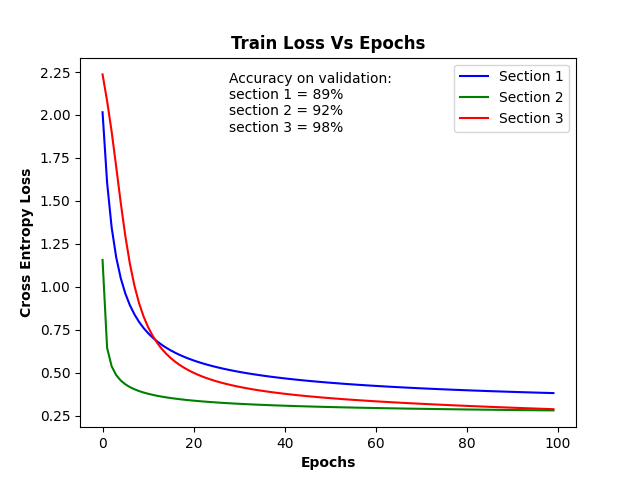
\includegraphics[width=0.5\textwidth]{train_loss_plots.png}
            \caption{Training loss curve. We can observe the faster convergence (in terms of epochs) of Section 2 compared to Section 1, as required.}
            \label{fig:figure_label}
        \end{figure}       
        
        
    \end{enumerate} % MNIST


\subsection{OpenAI Gym}
    \begin{enumerate} % OpenAI Gym
        \item done in the attached python file \textbf{gym\_cart\_pole.py}
        \item done in the attached python file \textbf{gym\_cart\_pole.py}
        \item done in the attached python file \textbf{gym\_cart\_pole.py}
        \item done in the attached python file \textbf{gym\_cart\_pole.py}
        \item done in the attached python file \textbf{gym\_cart\_pole.py}
        \begin{figure}[H]
            \centering
            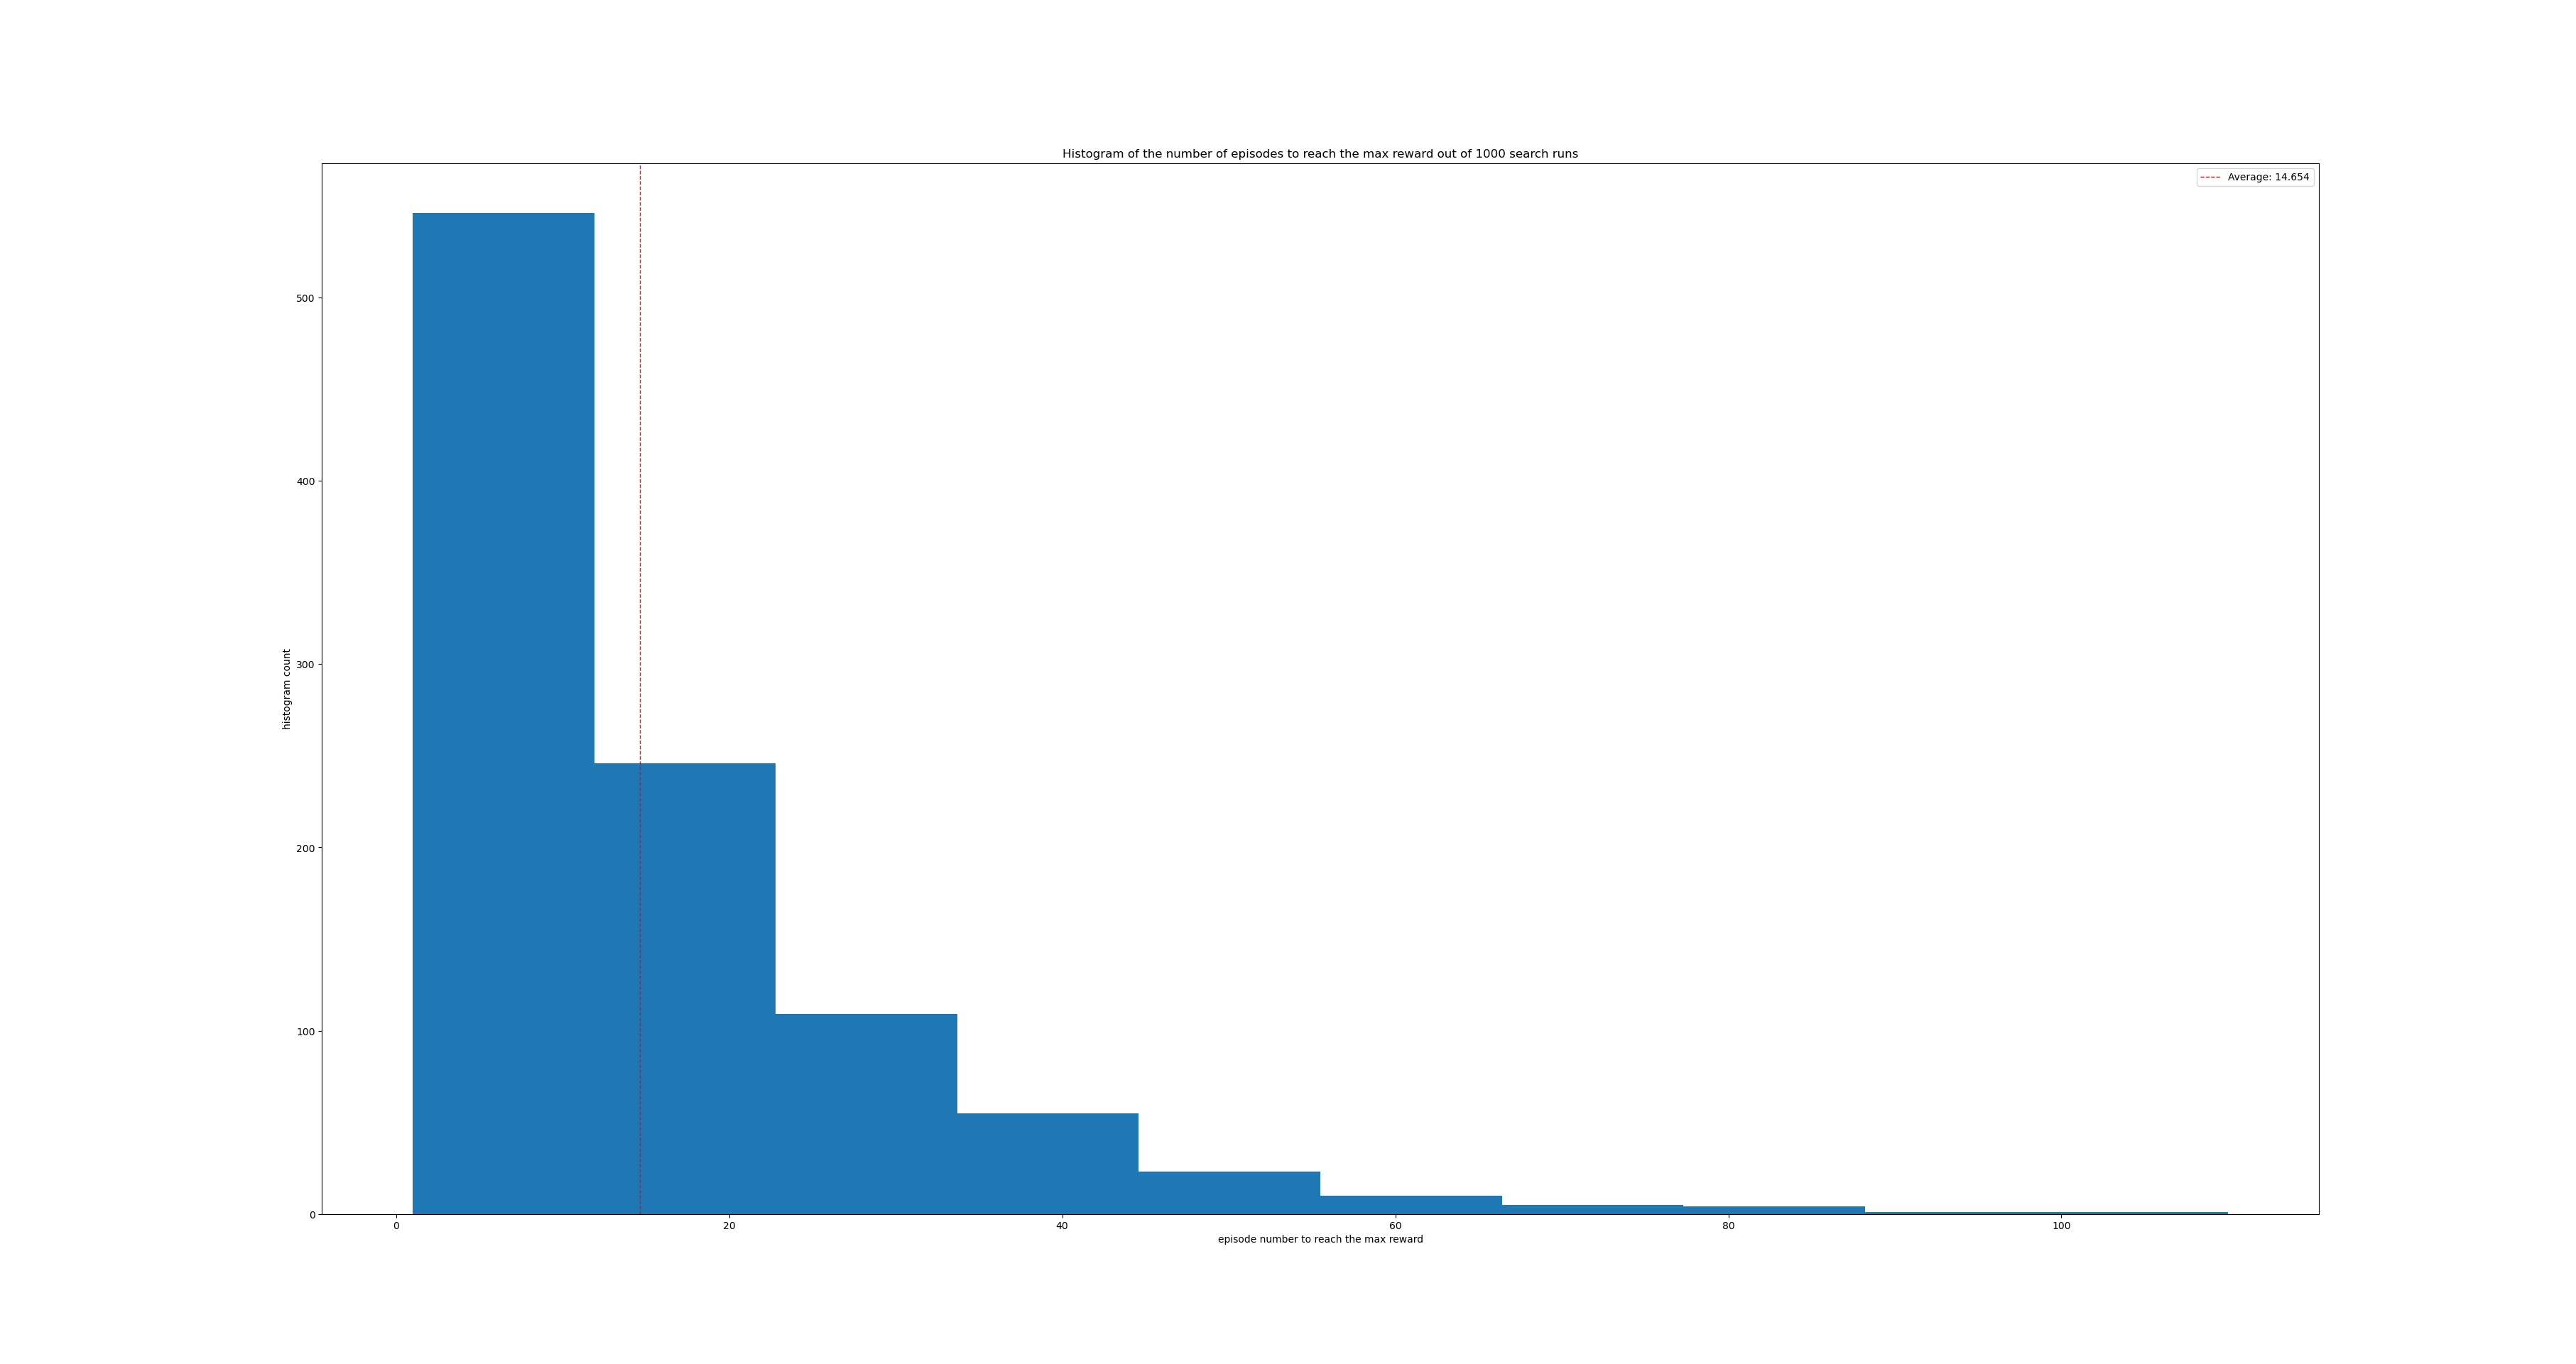
\includegraphics[width=0.5\textwidth]{4_2_5_hist.png}
            \caption{Histogram of the number of episodes to reach the max reward out of 1000 search runs, average is 14.65 episodes.}
            \label{fig:figure_label}
        \end{figure}
    \end{enumerate} % OpenAI Gym



\end{document}
